\documentclass[english]{article}
\usepackage[T1]{fontenc}
\usepackage[latin9]{inputenc}

\usepackage{geometry}
\geometry{verbose,tmargin=3cm,bmargin=3cm,lmargin=3cm,rmargin=3cm}
\usepackage{color}
\usepackage{babel}
\usepackage{refstyle}
\usepackage{float}
\usepackage{booktabs}
\usepackage{textcomp}
\usepackage{graphicx}
\graphicspath{{../figures/srs/}}
\usepackage[unicode=true,pdfusetitle,
 bookmarks=true,bookmarksnumbered=false,bookmarksopen=false,
 breaklinks=false,pdfborder={0 0 1},backref=false,colorlinks=true]
 {hyperref}

\usepackage{wrapfig}



% header
\title{HOSEA Aim I -- PPI, Anion Gap, Logistic Regression}
\author{Simon Fontaine}
\date{\today}

\begin{document}

\maketitle
\tableofcontents

\newpage
\clearpage
\section{Logistic Regression}

\textbf{Setting}
\begin{itemize}
\item I fitted a few logistic regression models with small changes in the
set of predictors to see how things change when we add/remove one
\item Known predictors: age, obesity (BMI>30), sex, gerd, smoking(any), white
\item Extra predictors: PPI (None, Low, High; cutoff: mean >20) and Anion gap (using the
mean of each component)
\item Age and Anion gap fitted using splines; everything is main-effects only
\item I also include the marginal models for comparison
\item A model with the interaction between PPI and anion gap (adjusting for all known
predictors also)
\end{itemize}
\textbf{Some notable observations:}
\begin{itemize}
\item Gerd seems to have an interaction with PPI but not the anion gap: indeed, including
only the anion gap doesn't change the estimate for Gerd much, but including PPI does
(maybe PPI is confounded by Gerd, which would be why we find PPI not to be important?)
\item Including the Anion gap changes PPI a little bit by decreasing the effect
\item Reversely, including PPI does change the Anion gap a little by attenuating the effect:
these two last observations would indicate some confounding between PPI and The Anion gap
\item PPI does seem to be associated with the outcome; there doesn't seem to be much of a difference between low and high (might be because of my definition)
\item PPI seem to amke the anion gap less variable?
\item There seems to be an interaction between PPI and anion gap: almost no effect of anion gap given no PPI. Unclear what is the difference with the main effect model only when looking at the peak.
\end{itemize}

\begin{figure}[h]
\centering
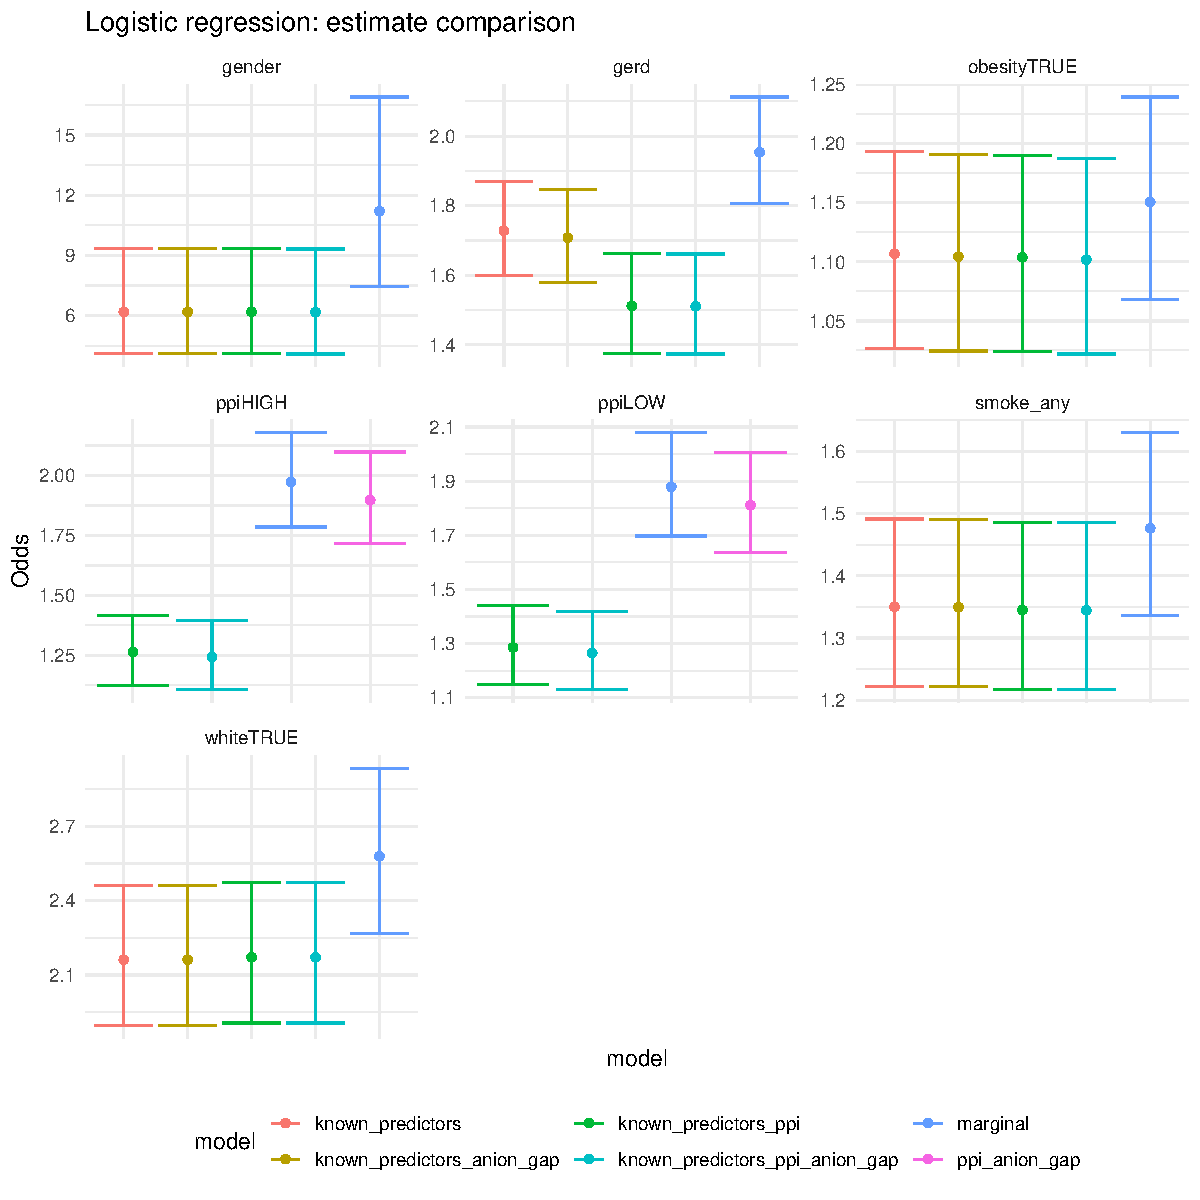
\includegraphics[width=\linewidth]{labs/logreg_coefs.pdf}
\end{figure}

\begin{figure}[h]
\centering
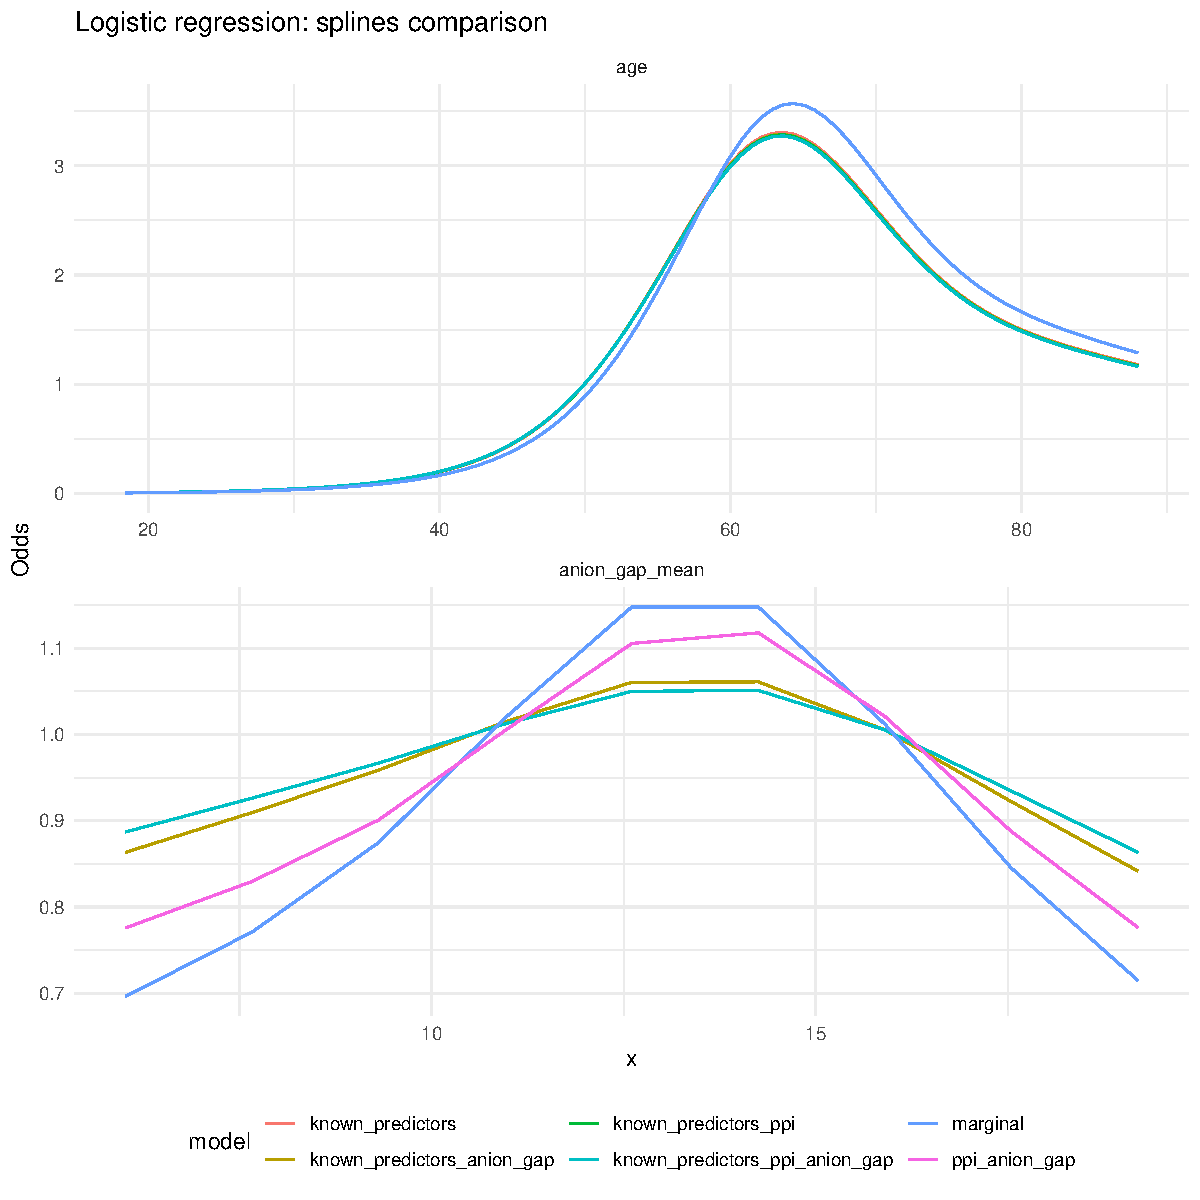
\includegraphics[width=\linewidth]{labs/logreg_splines.pdf}
\end{figure}

\begin{figure}[h]
\centering
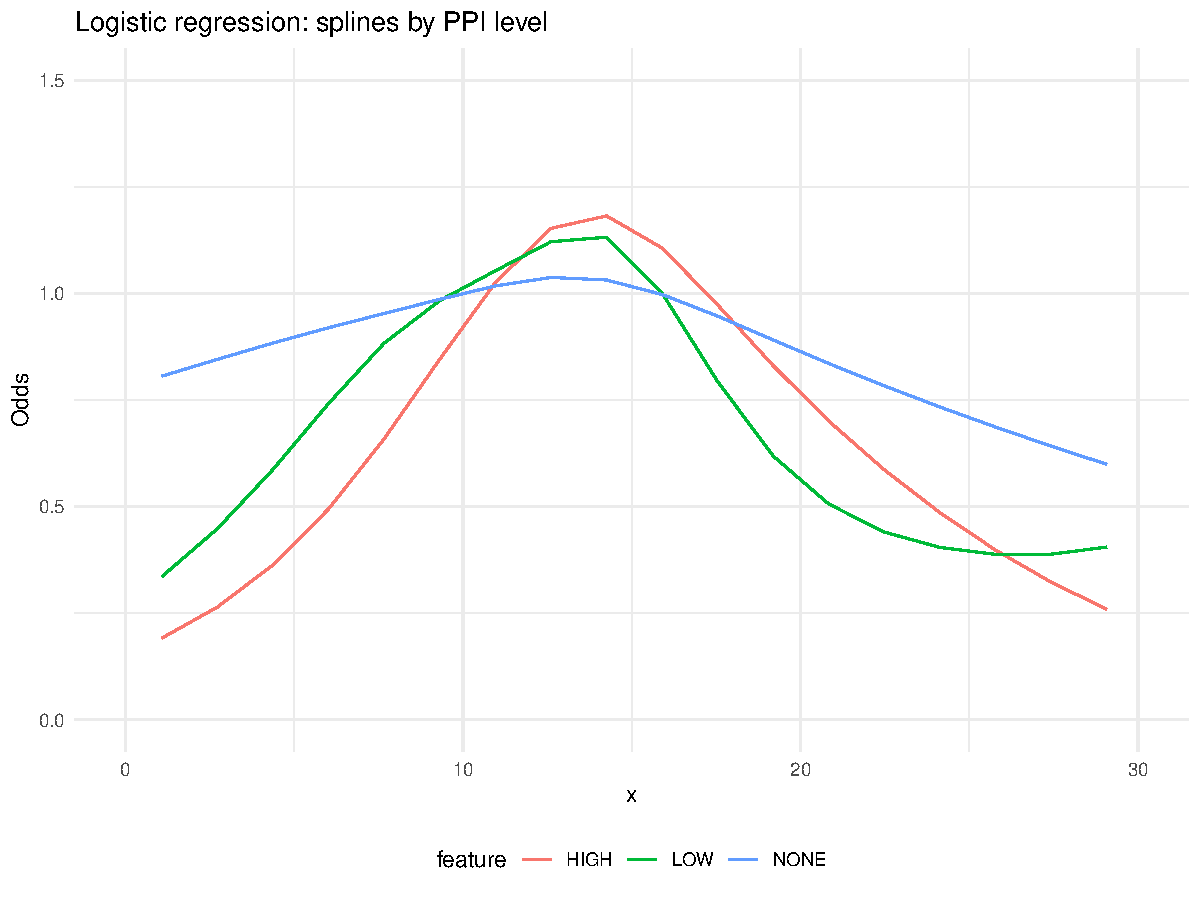
\includegraphics[width=\linewidth]{labs/logreg_splines_ppi_x_anion_gap.pdf}
\end{figure}

\end{document}
